\documentclass[12pt]{article}
\usepackage{geometry}                % See geometry.pdf to learn the layout options. There are lots.
\geometry{letterpaper}                   % ... or a4paper or a5paper or ... 
\usepackage{graphicx}
\usepackage{amssymb}
\usepackage{amsthm}
\usepackage{epstopdf}
\usepackage[utf8]{inputenc}
\usepackage[usenames,dvipsnames]{color}
\usepackage[table]{xcolor}
\usepackage{hyperref}
\usepackage{float}
\hypersetup{
    colorlinks=true,
    linkcolor=blue,
    filecolor=magenta,      
    urlcolor=cyan,
}
\usepackage{parskip}
\DeclareGraphicsRule{.tif}{png}{.png}{`convert #1 `dirname #1`/`basename #1 .tif`.png}

\theoremstyle{definition}
\newtheorem{example}{Example}

\newcommand{\projectname}{Doctor Robert}
\newcommand{\productname}{Doctor Robert}
\newcommand{\projectleader}{D. Weidinger}
\newcommand{\documentstatus}{In process}
%\newcommand{\documentstatus}{Submitted}
%\newcommand{\documentstatus}{Released}
\newcommand{\version}{v. 1.0}

\begin{document}
\begin{titlepage}
\begin{flushright}
\end{flushright}

\vspace{10em}

\begin{center}
{\Huge Project Proposal} \\[3em]
{\LARGE \productname} \\[3em]

\includegraphics[scale=.5]{logo.png}\\
\end{center}

\vspace{10em}

\begin{flushleft}
\begin{tabular}{|l|l|}
\hline
Project Name & \projectname \\ \hline
Project Leader & \projectleader \\ \hline
Document state & \documentstatus \\ \hline
Version & \version \\ \hline
\end{tabular}
\end{flushleft}

\end{titlepage}


\section*{Revisions}
\begin{tabular}{|l|l|l|}
\hline
\cellcolor[gray]{0.5}\textcolor{white}{Date} & \cellcolor[gray]{0.5}\textcolor{white}{Author} & \cellcolor[gray]{0.5}\textcolor{white}{Version/Change} \\ \hline
September 19, 2019&Weidinger, Gruber, Tanzer&First version \\ \hline
October 04, 2019&Weidinger, Gruber, Tanzer&Second version \\ \hline
October 07, 2019&Weidinger, Gruber, Tanzer&Third version \\ \hline
October 08, 2019&Weidinger, Gruber, Tanzer&Fourth version \\ \hline
October 10, 2019&Weidinger, Gruber, Tanzer&Final version 1.0 \\ \hline
October 21, 2019&Weidinger, Gruber, Tanzer&Final version 1.1 \\ \hline
October 24, 2019&Weidinger, Gruber, Tanzer&Final version 1.2 \\ \hline
\end{tabular}

\pagebreak


\tableofcontents

\pagebreak


\section{Introduction}
The end result of our project acts like a helping hand in the everyday life.
Instead of googling ones symptoms or complaints, the product uses a Machine-Learning Model, trained on medical data, to provide answers in the form of diagnoses and possible treatment plans. The product takes the user-input and computes possible solutions for ones disease.

\pagebreak


\section{Initial Situation}

When people start to show symptoms of a possible sickness or get mildly injured, they often tend to misjudge or downplay the severity of their conditions, to justify not making a doctors appointment, since going to the doctors is a big inconvenience for most people in this day of age. This behaviour often leads those people to seek out to google for a diagnosis.

Googling symptoms can be quite tedious and unnecessarily time-consuming. It involves opening a lot of sites, skimming trough loads of text and most of the time the results are rather inaccurate.

Although there are already good individual solutions for medical third opinions, there has yet to be a simple unified platform for all individual cases.

{\bf For example} \href{https://www.netdoktor.de/}{Netdoktor}, the market leader for medical articles and questions in German speaking countries, has a program called \href{https://www.netdoktor.de/symptom-checker/}{Symptom-Checker} that tries to simplify the process of searching for medical treatments on their own website by asking the user questions about their gender, age, area of pain, etc. This process also includes redundant questions and limits the user to input only by selection, which makes it hard to accurately describe symptoms. Netdoktor only supports the German language so if a user wants an English diagnosis they have to switch to a different service.

Such services also lack features like scanning skin in order to diagnose skin diseases, so a user has to use, or even download, another application like for example \href{http://www.skinvision.com}{Skin Vision}, which is a program used to recognize skin diseases based on images. This could lead the user to not look up their suspicious looking piece of skin. 

As of now we are not aware of any healthcare assistants or symptom checkers that make use of sophisticated Artificial Intelligence algorithms. Neuronal networks trained on medical data, like BioBert, already exist and outperform established solutions in regards of accuracy and convenience but are not easily accessible for the ordinary consumer.

\pagebreak


\section{General Conditions and Constraints}

{\large The proposed system has to the deal with the following conditions and constraints:}

\subsection{Confidentiality and Legality}
\vspace{2em}

{\bf We have to communicate that we are no substitute for a doctor}

To avoid legal consequences, the user needs to be informed that we take no responsibility for the diagnoses or information provided. Our competitors, namely NetDoktor, solved this problem by clarifying this before and while the interaction. Additionally, we have to shield ourselves from possible lawsuits by making the user to agree to our Terms of Service.
\vspace{2em}

{\bf All interactions with the user must be confidential}

Trust is one of the most important factor in the medical field. Nobody is willing to share their personal well-being when their is doubt in the confidentiality. This is why end-to-end encryption for user interactions is obligatory.

Even if we do not save medical data from our users, men-in-the-middle attacks are a possible threat. Attackers could potentially intercept data sent by the user. For example, ones employer could get their hands on a female workers pregnancy diagnose and fire her as a result.
\vspace{2em}

{\bf Personalize the experience with general information about the user}

The user, if wanted, signs-up for a more personalized experience. Depending on how the user is logged in, either anonymous or with an third party OAuth2 login like Google's, the user experience will slightly change in the way that he will for example be addressed by his name, the last time he logged in or other meta-information.
\vspace{2em}

\pagebreak


{\bf No medical data will be stored(For the moment)}

We currently do not have the capacity to deal with sensible data like medical information. Saving the personal medical data would be an additional legal threat, since we also cannot use it to improve our product we are not planning to take a risk in doing so. This could change in the future.
\vspace{2em}

\subsection{UX and technical constrains}

{\bf We have to be more convenient/precise than google when it comes to medical questions}

Otherwise, there would be no reason to use our product. 
\vspace{2em}

{\bf We have to avoid notoriety by giving false alarms so our critical evaluations like skin-cancer must be accurate}

It is easy to get a bad reputation in the medical field. One bad diagnosis can lead to an public outcry. This factor is especially important since our application is built on trust between the user and Doctor Robert, therefor our diagnoses have to be accurate.
\vspace{2em}

{\bf The output of our model must not be to technical and/or needs further explanation-methods like descriptions of medical terms}

Outputs like: "generally ekg will identify the long qt and brugada syndrome." need to be more readable. A lot of times the output text includes medical terms. For these words we have to provide further explanation.
\vspace{2em}

\pagebreak


\section{Project Objectives and System Concepts}

Our main goal is to represent a helpful third opinion. Potential users can ask Doctor Robert all questions regarding physical health and well being. The unbiased recommendations of Robert can then be used as is or for further research.

\subsection{Login}

The user, if wanted, signs-up for a more personalized experience. Depending on how the user is logged in, either anonymous or with an third party OAuth2 login like Google's, the user experience will slightly change in the way that he will be addressed by his name.

\subsection{Diagnosis}

\begin{minipage}{0.4\textwidth}
\begin{figure}[H]
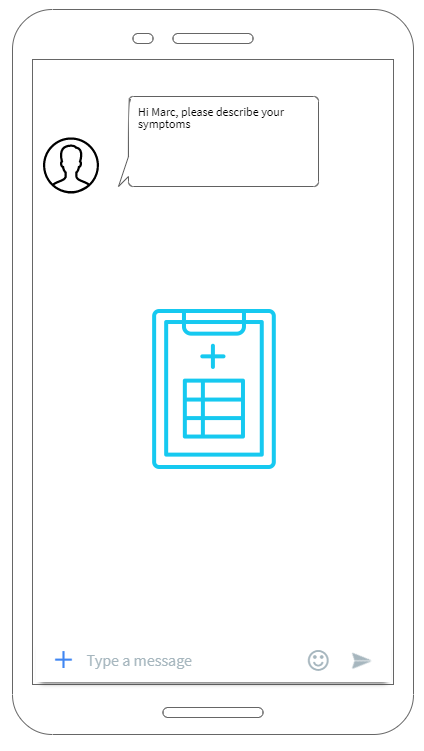
\includegraphics[scale=.45]{entwurf.PNG}\\
\caption{\label{fig:blue_rectangle} Prototype}
\end{figure}
\end{minipage} \hfill
\begin{minipage}{0.6\textwidth}

The user enters his ailments into the app. Using words or whole sentences to describe the current unwell-feeling. Since the predication will be more accurate if more keywords are read, a more precise description of the
illness is better than just words. Even though words alone are sufficient.

The output informs the user about possible symptoms causing the ill-being and/or about feasible solution and if desired further elaboration on certain results.

The user then can decide how to act from that point. Depending on the outcome he can leave it be, do further research through provided links or arrange a doctors appointment.

\end{minipage}

\subsection{Computer-Vision based Healthcare Tasks}

A picture taken by a user is used as base of operations for an elaborated computer vision algorithm. The algorithm can make viable diagnoses of the picture, thus about the state of the user. 
For example, skin irritations are scanned and then it is evaluated, whether the user has skin cancer or not.

Since such applications already exist around the world, the question Why self implement? may arise. The answer is fairly straight-forward. There are no services that actually provide integrable functionality. So self-implementation is practically forced.
    
On the contrary to the "Diagnosis tool", Computer-Vision based tasks will not be dealt with on the back-end, but locally on the mobile device. Since this will result in much lower server workload. 
    
\subsection{Readability and Language}

{\bf Translation}

The user interface will be available in multiple languages, mainly English. As the system is based in English, a translation is made to German or other languages via the Google translation API.

{\bf Keyword Recognition}

The given diagnoses often contain medical terms that are not understandable for the normal person. So, a redirection or further explanation has to be given for those appearances.
This will be resolved in a pop-up window that gives a short explanation and provides a link for further research.    
    
\subsection{Mobile-Application}

The mobile version features Login, "Diagnosis" telling and Computer-Vision Healthcare Tasks. The mobile-app and the web-app, both form the front-end. The mobile-app includes all functionalities stated above, whereas the web-app has to give up on the Computer-Vision Tasks. 
     
\subsection{Web-Application}

The web-app will be integrated in the website of the product. The overall experience for using the app remain relatively unchanged. The only downside it has against the mobile-app is the fact, that computer-vision scans like skin-cancer recognition will not be available due to the intricate integration of said functionality.
Otherwise the usability stays the same. "Diagnoses" can be made just like in the mobile version. 

\subsection{Back-End}

The back-end is mostly used as a REST API and for storing the users data, for the back-end consists of Google's Firebase and the REST API Server.
Also the AI based "Diagnosis" giving feature is seated in the back-end for a more efficient response time.


\pagebreak



\section{Opportunities and Risks}

\subsection{Google Alternative}

Our project presents the opportunity to form an user-base by enticing away people already using platforms like google to look up their symptoms, by providing a simpler way to get more accurate results. The process of googling can be simplified with the power of artificial intelligence. So a person does not have to dig trough various websites to get an fairly inaccurate medical diagnosis. The user will have an simple user-interface to enter their aches and pains and an accurate third medical opinion will be provided. 

\subsection{Unified Platform}

There are already working programs and methods for giving medical diagnoses. Which gives us the opportunity to embed those methods in our platform, since the general aim of our platform is to give the user the convenience of using only one platform to give them an accurate medical opinion.

\subsection{Notoriety}

It is critical for a system like ours to gain a good reputation and on the other hand to avoid bad notoriety for our predictions. About 70 percent of Americans say that online reputation had influenced their choice of physician(\href{https://www.mobihealthnews.com/content/95-americans-find-online-doctor-reviews-reliable-survey-suggests}{Source}). If Doctor Robert manages to get a good reputation, we could be a possible replacement for a google search. This implies a possible user-base of people equipped with internet-ready devices. The same holds true for the opposite. For example if our model gives a lot of wrong skin-cancer alarms, we could lose our reputation, respectively our relevancy.

\subsection{Intelligent advertisement}

One possible source of income could be advertisement of certain doctors for certain diagnoses in ones area. In order to back our claims of advertisement we would have to collect data on the usage of our application.
Like we declared in our Conditions and Constrain section, we do not store medical data. This is why the collection of the data has to be of statistical nature and purely anonymous.

\subsection{Legal risk}

First and foremost, it has to be said that the whole topic of AI supported medical treatments/diagnoses are intensely discussed in terms of the law. Up to now, no one, including experts, has come to the point of perspicuity - it is a grey-zone. Since we are no pioneers on the topic of digital medical diagnoses we know that it is legally possible.


\pagebreak


\section{Planning}

\subsection{Schedule}

Project begin: Mo, 14.10.2019\\
Project end: End of 5th grade\\

Our first hurdle will be the setup for our back-end. Parallel we will start to develop a front-end. The development will start with the 4th of November.

The first working prototype is set to be available by the end of the first semester. 

\subsection{Management}

For software development we will be using Scrum as the method for managing and tracking development process. 

\subsubsection{Team}
    {\bf Daniel Weidinger}:
    \begin{itemize}
        \item Role: Teamleader
        \item Focus: Back-End and AI development
    \end{itemize}
    As a team leader the duty is neat and efficient course of action over the whole project. Thus required to ensure a fluent and communicative team work.\\
    In charge of the development of the back-end and AI services.
    
    \vspace{1em}
    {\bf Jan Gruber:}
    \begin{itemize}
        \item Role: Developer
        \item Focus: Front-End
    \end{itemize}
    As the leading role in the Front-End development the main focus is in creating a clean app and website. Also partly operating in the AI development. 
    
    \vspace{1em}
    {\bf Rafael Tanzer:}
    \begin{itemize}
        \item Role: Developer
    \end{itemize}
    Applying and working in all fields(back-end, front-end and AI).
    Main emphasis on back-end and AI and posing as a sort of intermediary between Front-End and Back-End development.
    
\subsubsection{Versioning}

    The price for every used product will be provided in the parenthesis after the name

    Versioning: Git({\bf free}) - Git is a distributed version-control system for tracking changes in source code during software development. 
    
    Repository: GitHub({\bf free}) - GitHub is an American company that provides hosting for software development version control using Git
    
    Git GUI Client: GitKraken({\bf free}) -  GitKraken is an intuitive and seamless UI for git
    
\subsubsection{Other organisational software}

    Scrum Board: GitKraken GLO({\bf free}) - GitKraken Glo is the only incandescent issue board for task and issue tracking that is fully integrated with GitKraken. 

\pagebreak
\subsubsection{Resources}
    
    The price for every used product will be provided in the parenthesis after the name
    
    {\bf IDEs and Development Platforms:}
    
    \begin{itemize}
        \item JetBrains's Android Studio + Flutter and Dart Plugin ({\bf free})
        \item Visual Studio Code ({\bf free}) 
        \item Python 3 Interpreter ({\bf free})
    \end{itemize}
    
    {\bf Backend:}
    \begin{itemize}
        \item Firebase for user-data storage({\bf free up to a certain point then we pay per usage.})
        \item Server with an Python runtime for REST calls ({\bf free up to a certain point if we do not use it commercially})
        \item Tensorflow Serving for faster machine-learning inference. ({\bf free})
        \item Google Translation API ({\bf free up to a certain point})
    \end{itemize}
    
    {\bf Frontend:}
    \begin{itemize}
        \item Access to the Google developer console in order to make our application available ({\bf 20 Euro})
    \end{itemize}
    
\pagebreak
    
   
\subsection{Milestones}

This section lists a brief overview of our most crucial milestones.

\begin{left}
    \begin{tabular}{ | m{6cm} | m{2cm}| m{8cm} | } 
    \hline
    \cellcolor[gray]{0.5}\textcolor{white}{Milestone} & \cellcolor[gray]{0.5}\textcolor{white}{Date} & \cellcolor[gray]{0.5}\textcolor{white}{Description} \\ \hline
    \hline
    Mobile application & 31.12.2019 & Cross-platform mobile application(Android/IOS) which can communicate with our back-end \\ 
    \hline
    User (Login/Register) integration  & 14.2.2020 & back-end and front-end integration of a login feature and a user database \\
    \hline
    REST API & 14.2.2020 & Working REST API for our DocNet(our Neuronal Network) \\ 
    \hline
    Skin Cancer Recognition & 31.04.2020 & functionality for a camera based inference to recognize skin cancer.\\ 
    \hline
    Explanation of medical terms & 31.6.2020 & Based on certain medical keywords we provide further explanation \\ 
    \hline
    Web front-end & 31.10.2020 & Web front-end with the same functionality as the mobile font-end expect the computer-vision tasks \\ 
    \hline
    \end{tabular}
\end{left}


\pagebreak


\section{List of Abbreviations}

\begin{itemize}
    \item UI ... User Interface
    \item AI ... Artificial Intelligence
    \item UX ... User Experience
\end{itemize}

\end{document}  